% Be sure to address the following items:
% -   Introduction
% -   Define sequence of tasks to be performed
% -   Identify all deliverables (Milestone Deliveries)  - IMPORTANT:  This is a
%     critical item in that your future deliveries will be evaluated based on
%     this.   It needs to be clear, detailed, and objective (can I go through
%     your milestone description like a check list to see if your delivery is
%     complete?).   Note, as the project goes forward this can change, and that
%     is perfectly OK.
% -   Define the dependency relationship between each task
% -   Estimate resources required to perform each task
% -   Schedule all tasks to be performed
% -   Define the organization executing the project
% -   Identify the known project risks (Risk Analysis)
% -   Define the process to ensure quality (Test Plan)
% -   Define the process for configuration management
% -   Define the process specifying and controlling the design requirements




\documentclass[12pt,titlepage]{article}
\usepackage[margin=1.0in]{geometry}
\usepackage{graphicx}
\usepackage[pdftex]{hyperref}
\usepackage[english]{babel}
\usepackage{csquotes}
\usepackage{titling}
\usepackage{titlesec}
\usepackage{tabularx}
\usepackage{float}
\usepackage{xspace}
\usepackage{tabularx}
\usepackage{parskip}

\usepackage{enumitem,amssymb}
\newlist{todolist}{itemize}{2}
\setlist[todolist]{label=$\square$}

\usepackage{pifont}
\newcommand{\cmark}{\ding{51}}%
\newcommand{\xmark}{\ding{55}}%
\newcommand{\done}{\rlap{$\square$}{\raisebox{2pt}{\large\hspace{1pt}\cmark}}%
\hspace{-2.5pt}}

\newcommand\tab[1][.5in]{\hspace*{#1}}
\newcommand\gametitle{\textit{\AE on Chronicles}\xspace}

\title{Project Plan}
\author{Team Epsilon}
\date{\today}

\begin{document}
\maketitle

\section{Introduction}

This document outlines the project management guidelines for Team Epsilon's
development of \gametitle, an adventure RPG video game.

The rest of the document is organized as follows. Section~\ref{sec:tasks}
outlines the tasks that will be performed at each milestone, what dependencies
exist between the tasks, and what the task schedule will be.
Section~\ref{sec:org} explains the organization of the team.
Section~\ref{sec:dev} outlines the development process including what documents
will be maintained and a test plan to ensure game quality.

\section{Tasks}
\label{sec:tasks}
This section outlines the tasks that must be completed to ensure that the
development of \gametitle is successful.

\subsection{Milestone Deliveries}
\begin{todolist}
\item[\done] \textbf{Milestone I:} Overworld
    \begin{todolist}
    \item[\done] Character Movement
    \item[\done] NPC interaction
    \item[\done] Combat Hooks
    \item[\done] Menu UI Systems
    \end{todolist}

\item[\done] \textbf{Milestone II:} Combat System
    \begin{todolist}
    \item[\done] Deck Randomization
    \item[\done] Turn Based System
    \item[\done] Combat Animations
    \item[\done] End of combat (apply damage)
    \end{todolist}

\item[\done] \textbf{Milestone III:} Alpha Release
    \begin{todolist}
    \item[\done] Integrate Overworld and combat
    \item[\done] Story flushed out
    \item[\done] A working location
    \item[\done] Sound Assets
    \end{todolist}

\item \textbf{Milestone IV:} Beta Release
    \begin{todolist}
    \item All regions of world
    \item Asset Integration
    \item Pool of approximately 30 cards per character
    \item 30 non-character specific cards
    \item Minimum of 4 elemental status types
    \item Card Crafting
    \item Music
    \end{todolist}

\item \textbf{Milestone V:} Final Release
    \begin{todolist}
    \item bug fixes
    \item stretch goals
    \end{todolist}
\end{todolist}

\subsection{Dependencies \& Resources}
Table~\ref{tab:dependencies} outlines the major dependencies between the tasks
in our project.
\begin{table}[H]
    \caption{Dependencies}
    \label{tab:dependencies}
    \centering
    \begin{tabularx}{\linewidth}{|l|X|}
        \hline
        \textbf{Task} & \textbf{Dependent Tasks} \\
        \hline
        Character Movement in Overworld & NPC Interaction, Combat Hooks \\
        \hline
        Turn Based Combat System & End of Combat (apply damage), Overworld and
        Combat Integration \\
        \hline
        Card Design & Card Enhancement behavior via Elements Mechanic, Card Crafting \\
        \hline
        Flesh Out Story & A working location \\
        \hline
    \end{tabularx}
\end{table}

\subsection{Task Schedule}
Table~\ref{tab:schedule} shows the timetable for milestone completion.
\begin{table}[H]
    \caption{Milestone Delivery Schedule}
    \label{tab:schedule}
    \centering
    \begin{tabular}{|l|l|}
        \hline
        \textbf{Milestone} & \textbf{Date} \\
        \hline
        Milestone I: Overworld & 2017/02/27 \\
        \hline
        Milestone II: Combat & 2017/03/13 \\
        \hline
        Milestone III: Alpha & 2017/03/24 \\
        \hline
        Milestone IV: Beta & 2017/04/14 \\
        \hline
        Milestone V: Final & 2017/04/26 \\
        \hline
    \end{tabular}
\end{table}

Figure~\ref{fig:gantt} shows our project schedule in the form of a Gantt chart.

\begin{figure}[H]
    \caption{Gantt Chart}
    \label{fig:gantt}
    \centering
    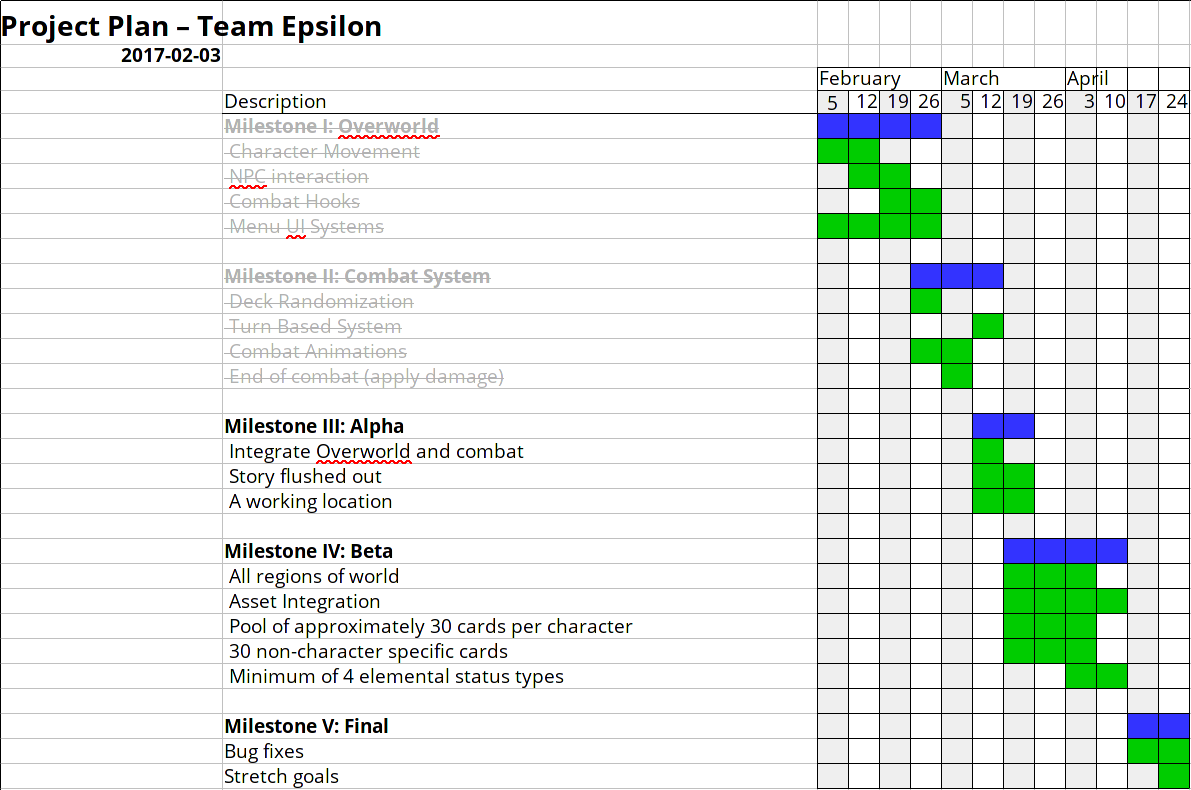
\includegraphics[width=\textwidth]{gantt-chart}
\end{figure}

\section{Organization}
\label{sec:org}
Each team member has a specific set of tasks described below. In addition to
their individual tasks, all team members will contribute to the coding effort.
\begin{itemize}
    \item \textbf{Caleb:} Recorder and Scheduler, Programming, Test Lead
    \item \textbf{David:} Programming, Story Creation
    \item \textbf{Jacob:} Programming, Sound \& Music
    \item \textbf{Robbie:} Team Lead, Concept Art, Programming
    \item \textbf{Sumner:} Programming, Document Maintenance
\end{itemize}

\section{Development}
\label{sec:dev}

\subsection{Documents}

Table~\ref{tab:dev_docs} is a list of documents relevant to maintaining the project.

\begin{table}[H]
    \centering
    \caption{Development Documents}
    \label{tab:dev_docs}
    \begin{tabularx}{\linewidth}{|l|X|}
        \hline
        {\bf Document}         & {\bf Purpose} \\ \hline
        {\it Design Document}  & The design document is a detailed blueprint on every
        aspect of the game. \\ \hline
        {\it Bugs \& Features} & Documents all upcoming and completed features, as well
        as descriptions and discovery-dates of all bugs for a
        particular feature. A status is provided for each
        feature which indicates whether the feature has been
        tested by the Test Lead for further bugs. Each bug
        includes a Resolution field that indicates whether the
        bug has been resolved, as well as a description as to
        how the bug was resolved. \\ \hline
    \end{tabularx}
\end{table}


\subsection{Risk Analysis}

Table~\ref{tab:risks} lists all possible major risks of the project and
our contingency plans to avoid each issue and what we will do in the case that
it occurs.

\begin{table}[H]
    \caption{Risk Analysis}
    \label{tab:risks}
    \centering
    \begin{tabularx}{\linewidth}{|l|X|}
        \hline
        \textbf{Possible Risk} & \textbf{Contingency Plan} \\
        \hline
        Non-competitive enemy AI & If it proves too difficult to create
        different AIs for various enemies and bosses, we can opt to create only
        one enemy AI to use with every combat encounter. We can also make this
        more simple than we'd like to save time. \\
        \hline
        Overambitious project scope & We believe that we have allocated our
        milestone goals in a way that we will be able to implement the core
        gameplay and assets that are necessary for the game to function;
        however, it is possible that we have been overambitious in our
        allocations. If that is the case we will have to cut back on
        functionalities and assets starting with in depth art and music assets
        followed by unique cards and encounters in tandem with overworld
        locations and interactions. This could also limit story development.  \\
        \hline
        Meeting deadlines & This risk has many similarities to the risk of an
        overambitious project scope. If we are unable to integrate a desired
        functionality before a milestone delivery, we will table the
        functionality until we have extra time to complete it in addition to all
        other parts of the next delivery. This could result in it being tabled
        indefinitely in which case we will refer to the order of functionalities
        to drop described above. \\
        \hline
        Large number of dependencies between tasks & We believe we have
        allocated our milestone goals in a way that we will be able to implement
        the necessary functionalities prior to when we plan to implement the
        functionalities that depend on them. If that is not the case, similarly
        to the case of not meeting deadlines, we will drop functinalities in the
        order described above. \\
        \hline
    \end{tabularx}
\end{table}

\subsection{Test Plan}

In general, periodic plays and replays of sections of the game should be done to
provide a loose redundant check on the game's stability. A more formal testing
structure is defined next.

Testing of the game will take place in incremental steps throughout development
of the game. While automated testing would present a robust and consistent
testing method, the time constraints of the project and its nature as a video
game make this an infeasible testing strategy. Therefore, the team will rely on
a system of collaborative manual testing that works as follows:

\begin{enumerate}
    \item When adding a new feature to the game, the developer(s) adding the
        feature will test it and ensure that all directly affected aspects of
        the game perform in the expected manner. The feature will then be
        documented in the {\it Bugs \& Features} document. Any remaining bugs
        that the developer is unable to resolve should also be documented in the
        {\it Bugs \& Fixtures} document.
    \item It is then up to the Test Lead to monitor the {\it Bugs \& Features}
        document for new features that they should test for completeness and
        bugs.  If the Test Lead is unable to resolve all bugs for any reason,
        they may delegate specific bug resolutions to other members of the team.

        {\it Caveat}: In the case that the Test Lead has added a particular
        feature themselves, they must act in accordance with step 1. The task of
        further testing (step 2) then falls on the Team Leader by default,
        though the Test Lead may assign this to another team member at their own
        discretion on a case-by-case basis.
\end{enumerate}

\subsection{Configuration Management}
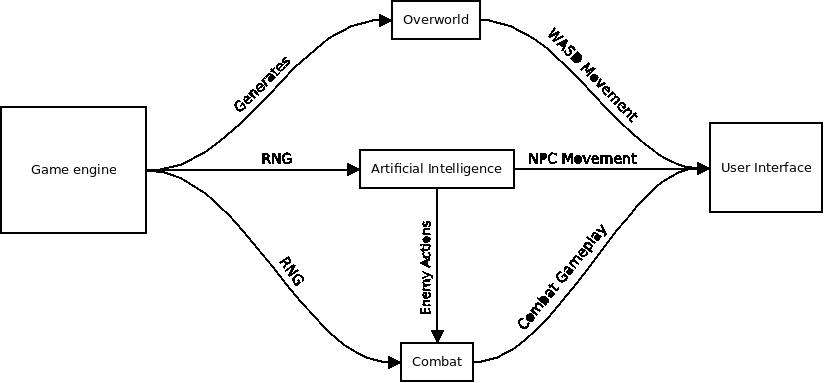
\includegraphics[width=16cm]{config-management}

\subsection{Design Requirement Update Procedure}

If any member of the team wants to change the design, the following steps must
be followed.

\begin{enumerate}
    \item The person who wants to change the design will notify the rest of the
        team and explain the change.

    \item If there is immediate consensus, or if it is a minor change, the
        person who proposed the change can proceed with the change (see 4).

    \item If there is not immediate consensus, a vote will be held and if a
        majority of the team members approve the change, the person who proposed
        the change can proceed with the change.

    \item After the change is approved by the team, the person who proposed the
        change has the responsibility of updating the design document with said
        change or delegating the task to another willing team member.

    \item After the Design Document has been updated, the Document Maintainer
        (Sumner) will be notified and he will ensure that the change fits the
        document organization.
\end{enumerate}

\end{document}
